\documentclass[final]{beamer}
\usepackage{grffile}
\mode<presentation> {
\usetheme{XDI}
\setbeamercovered{transparent}
}

\usepackage{color,fancybox,alltt,graphicx,listings}
\usepackage{type1cm,calc,times,amsmath,amsthm, amssymb, latexsym}

\boldmath
\usepackage[english]{babel}
\usepackage[latin1]{inputenc}
\definecolor{Red}{rgb}{0.5,0,0}
\definecolor{Blue}{rgb}{0,0,0.75}
\newcommand{\Color}[2]{{\textcolor{#1}{#2}}}
\newcommand{\Red}[1]{{\Color{Red}{#1}}}
\newcommand{\EmphRed}[1]{{\Color{Red}{\emph{#1}}}}
\newcommand{\BoldRed}[1]{{\Color{Red}{\bf{#1}}}}


\newcommand{\Blue}[1]{{\Color{Blue}{\bf{#1}}}}

\usepackage[orientation=portrait,size=a0,scale=1.4]{beamerposter}
\graphicspath{{images/}}

\title[XAFS Data Formats Poster]{Efforts toward Data Format Standardization for X-ray Absorption Spectra}
\author[Newville, Sol\'e, Ravel, and Hester]{
Matthew Newville${}^{a}$, V. Armando  Sol\'e${}^{b}$,  James R. Hester${}^{c}$, and Bruce Ravel${}^{d}$}
\institute[]{ 
  ${}^{a}$Center for Advanced Radiation Sources, University of  Chicago, USA, \par
  ${}^{b}$European Synchrotron Radiation Facility, Grenoble, France, \par
  ${}^{c}$Bragg Institute, Australian Nuclear Science and Technology Organization, Kirrawee, Australia, \par
  ${}^{d}$National Institute  of Standards and Technology, Gaithersburg,
  USA
}

  \date{23-July-2012}
  
  \begin{document}
  \begin{frame}{}
    \vspace{2mm}
    \begin{columns}[t]
      \begin{column}{.52\linewidth}
        \begin{block}{\large Abstract}

          In order to address the need for easier exchange and archiving of
          X-ray absorption data, we propose a data format for spectra of
          $\mu(E)$ using a simple plaintext file, and invite comments and
          discussion. The XAS Data Interchange (XDI) format uses
          space-delimited columns for numerical absorption data, and so is
          similar to that currently used at many facilities, but with a
          well-defined structure for metadata in the file header.  Several
          example XDI files and programming libraries for reading these
          files are shown, and made publicly available.  Because this data
          format can accommodate only single spectra, we also discuss
          methods for combining multiple spectra into spectral libraries
          using either hierarchical data format (HDF5) or using relational
          databases based either on the CIF format or SQL-based database
          engine.

        \end{block}
        
        \vspace{2mm}
        
        \begin{block}{\large X-ray Data Interchange Format}
        
          {\Red{Motivation here :   NEEDS WORK}}
          
          
          Storing and Exchanging XAFS Data is a common need for everyone
          using XAFS.  In particular, retrieving data on ''Standards'' or
          ''Model Compounds'' is a continuing need for both XANES and EXAFS
          analysis.  Additionally, data taken on samples at different
          facilities and beamlines need to be compared and analyzed together.
          At this point, there is no commonly accepted data format for XAFS
          data.  There have been a few attempts to standardize the
          traditional "ASCII Column File".  To be sure, ASCII Column Files
          have some strong appeal. Most data collection software saves such
          files, and most processing and analysis software use some variation
          of this format.  In addition, such files may be easily read by
          humans and used in a wide variety of third party
          applications. Still, most ASCII Column Files need some intimate
          knowledge of the data layout to use the data.  The lack of a
          standard ASCII format is a serious problem. The work here is
          parallel to the efforts to come up with a standard. and will be
          able to convert data into such standard file formats.
          

          \begin{center}
            \begin{minipage}[t]{0.5\linewidth}
              \large $\mu(E)$ is the basic spectra
            \end{minipage}
          \end{center}

          More text

        \end{block}
      \end{column}
      \begin{column}{.45\linewidth}
        \begin{block}{Example XDI File}
          \begin{center}
            \begin{minipage}[t]{0.95\linewidth}
              \begin{alltt}
                {\footnotesize
                  \#XDI/1.0  {\BoldRed{$\leftarrow$ Version Info}}\par
                  \#Beamline.name: APS 10ID\par
                  \#Mono.name:  Si 111\par
                  \#Mono.d\_spacing: 3.13553\par
                  \#Element.symbol: Fe\par
                  \#Element.edge: K\par
                  \#Column.1: energy eV    
                  {\BoldRed{$\leftarrow$ Column Labels, Units}}\par
                  \#Column.2: mutrans\par
                  \#Column.3: i0\par
                  \#///
                  {\BoldRed{$\leftarrow$ start multi-line comment}}\par
                  \#Fe K-edge, Lepidocrocite powder\par
                  \#on 4 layers of tape\par
                  \#------- {\BoldRed{$\leftarrow$ End Header, Begin Arrays Table}}\par
                  \#\par
                  \hspace{3mm} 6899.9609 -1.3070486 149013.70\par
                  \hspace{3mm} 6900.1421 -1.3006104 144864.70\par
                  \hspace{3mm} 6900.5449 -1.3033816 132978.70\par
                  \hspace{3mm} 6900.9678 -1.3059724 125444.70\par
                  \hspace{3mm} \ldots\par
                }
              \end{alltt}
            \end{minipage}
          \end{center}
        \end{block}

        \vspace{2mm}
        \begin{block}{\large XDI File description}

 
         Required metadata (case insensitive):

          \begin{itemize}
            \item {\Blue{Element.symbol}}  Atomic symbol of absorbing element
            \item {\Blue{Element.edge}}    K, L3, M4, etc
            \item {\Blue{Mono.d\_spacing}}  Strongly encouraged for all data,
              required if mono angle is given and mono energy is not.
          \end{itemize}

          \vspace{3mm}

          \hrule

          \vspace{3mm}

          Supported column labels.  These labels for Columns should
         be used, and may be required for certain data sets.
         
         \begin{itemize}
         \item {\Blue{\tt{energy}}}  Monochromator energy, in eV or keV.
         \item {\Blue{\tt{angle}}}   Monochromator angle, in degrees.
         \item {\Blue{\tt{i0}}}
         \item {\Blue{\tt{time}}}
         \item {\Blue{\tt{itrans}}}
         \item {\Blue{\tt{ifluor}}}
         \item {\Blue{\tt{irefer}}}
         \item {\Blue{\tt{mutrans}}}
         \item {\Blue{\tt{mufluor}}}
         \item {\Blue{\tt{murefer}}}
         \item {\Blue{\tt{normtrans}}}
         \item {\Blue{\tt{normfluor}}}
         \item {\Blue{\tt{normrefer}}}
         \item {\Blue{\tt{k}}}
         \item {\Blue{\tt{chi}}}
         \end{itemize}

          \vspace{6mm}

          Table of metadata fields and meanings
 % ;
 
        \end{block}
      \end{column}
    \end{columns}
    \vfill

    \begin{block}{Options for Storing and Managing Multiple XDI Spectra}

      XDI describes exactly one XAFS $\mu(E)$ or $\chi(k)$ spectra.
      Obviously, having a community standard for storing and managing
      libraries of spectra would be useful.   

      \vspace{5mm}

      Below are three options that could be used to hold multiple spectra,
      and be able to read / write to XDI files.

      {\Red{ each needs more explanation!}}

    \end{block}

    \begin{columns}[t]
      \begin{column}{.32\linewidth}
        \begin{block}{HDF5 -- Heierarchical Data Format}

        {\centering
          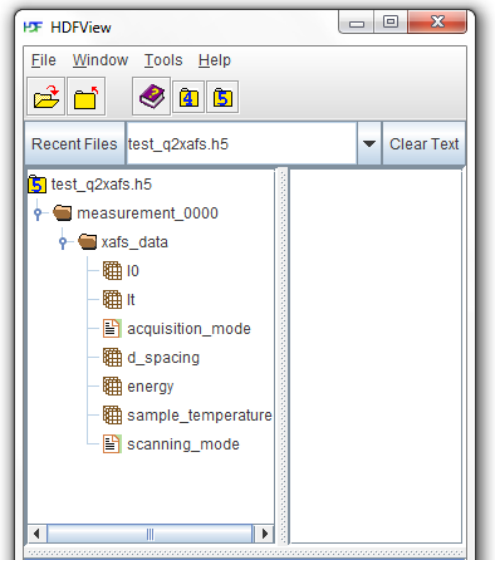
\includegraphics[height=0.8\linewidth]{hdf5.png}
        }
        
        
        \end{block}
      \end{column}
      \begin{column}{.32\linewidth}
        \begin{block}{CIF -- Crystallographic Information File}

          {\centering \begin{minipage}{0.8\linewidth}
              \begin{alltt}
                {\tiny
                  data\_v2o5\_nanotube\par
                  \_xafs\_absorber.atom   V\par
                  \_xafs\_absorber.edge    K\par
                  \_xafs\_source.identification   'KEK-PF BL20B'\par
                  \_xafs\_source.location         'Tsukuba, Japan'\par
                  loop\_\par
                  \_xafs\_detectors.label\par
                  \_xafs\_detectors.position\par
                  \_xafs\_detectors.type\par
                  monitor      monitor    ionisation\par
                  io-detector  detector   ionisation    foil         foil       ionisation\par
                  \par
                  loop\_\par
                  \_xafs\_ionisation\_detector.label\par
                  \_xafs\_ionisation\_detector.gas\_pressure\par
                  \_xafs\_ionisation\_detector.length\par
                  \_xafs\_ionisation\_detector.amplifier\_type\par
                  \_xafs\_ionisation\_detector.amplifier\_gain\par
                  monitor         1      10    'Keithley'    10\par
                  io-detector     1      20    'Keithley'    10\par
                  foil            1      5     'Keithley'    11\par
                  \par
                  loop\_\par
                  \_xafs\_reduced.energy\par
                  \_xafs\_reduced.absorbance\par
                  5248.52108 0.813707373\par
                  5258.29435 0.798733337\par
                  5268.26606 0.781069442\par
                  5278.27878 0.764530778\par
                  5288.28697 0.748170706\par
                  5298.19834 0.731395959\par
                  \ldots\par
                }
              \end{alltt}
              \end{minipage} }
        \end{block}
      \end{column}

      \begin{column}{.32\linewidth}
        \begin{block}{SQLite -- relational database in a file}

        {\centering
        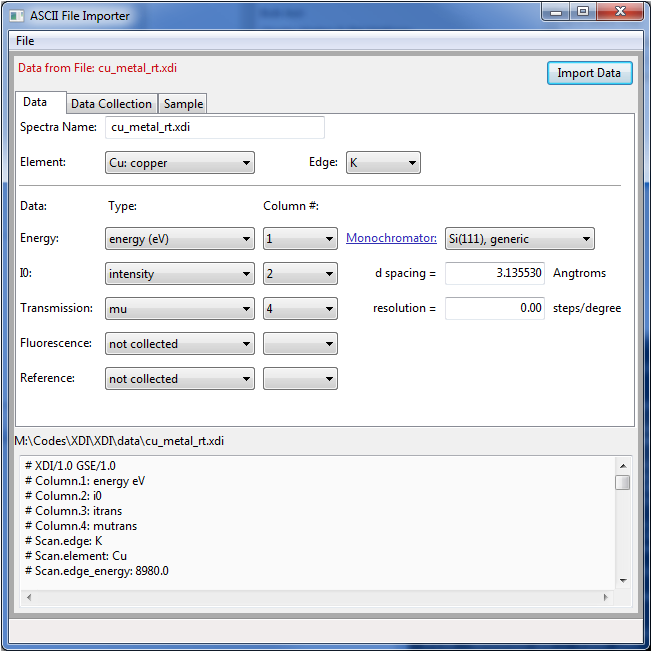
\includegraphics[height=0.8\linewidth]{sqlite.png}
      }
        \end{block}
      \end{column}

    \end{columns}
  \end{frame}
\end{document}
